\documentclass{article}

%----------------------------------------------------------------------------------------
%	PACKAGES AND OTHER DOCUMENT CONFIGURATIONS
%----------------------------------------------------------------------------------------

\usepackage{amsmath,amsfonts,stmaryrd,amssymb} % Math packages
\usepackage{enumerate} % Custom item numbers for enumerations
\usepackage[ruled]{algorithm2e} % Algorithms
\usepackage[framemethod=tikz]{mdframed} % Allows defining custom boxed/framed environments
\usepackage{textcomp}
\usepackage{float}
\usepackage{biblatex}
\usepackage{listings} % File listings, with syntax highlighting
\usepackage{graphicx}
\usepackage{hyperref}

\makeatletter
\newcommand{\addloflink}[1]{% \addloflink{<URL>}
  \addtocontents{lof}{\begingroup\def\protect\@dotsep{10000}% Remove dots in LoF for this entry
    \protect\contentsline{figlink}{\protect\numberline{}\url{#1}}{}{}%
    \endgroup}% Restore dots in LoF for future entries
}


%----------------------------------------------------------------------------------------
%	DOCUMENT MARGINS
%----------------------------------------------------------------------------------------

\usepackage{geometry} % Required for adjusting page dimensions and margins

\geometry{
	paper=a4paper, % Paper size, change to letterpaper for US letter size
	top=2.5cm, % Top margin
	bottom=3cm, % Bottom margin
	left=2.5cm, % Left margin
	right=2.5cm, % Right margin
	headheight=14pt, % Header height
	footskip=1.5cm, % Space from the bottom margin to the baseline of the footer
	headsep=1.2cm, % Space from the top margin to the baseline of the header
	%showframe, % Uncomment to show how the type block is set on the page
}

%----------------------------------------------------------------------------------------
%	FONTS
%----------------------------------------------------------------------------------------

\usepackage[utf8]{inputenc} % Required for inputting international characters
\usepackage[T1]{fontenc} % Output font encoding for international characters

\usepackage{XCharter} % Use the XCharter fonts

%----------------------------------------------------------------------------------------
%	COMMAND LINE ENVIRONMENT
%----------------------------------------------------------------------------------------

% Usage:
% \begin{commandline}
%	\begin{verbatim}
%		$ ls
%		
%		Applications	Desktop	...
%	\end{verbatim}
% \end{commandline}

\mdfdefinestyle{commandline}{
	leftmargin=10pt,
	rightmargin=10pt,
	innerleftmargin=15pt,
	middlelinecolor=black!50!white,
	middlelinewidth=2pt,
	frametitlerule=false,
	backgroundcolor=black!5!white,
	frametitle={Command Line},
	frametitlefont={\normalfont\sffamily\color{white}\hspace{-1em}},
	frametitlebackgroundcolor=black!50!white,
	nobreak,
}

% Define a custom environment for command-line snapshots
\newenvironment{commandline}{
	\medskip
	\begin{mdframed}[style=commandline]
}{
	\end{mdframed}
	\medskip
}

%----------------------------------------------------------------------------------------
%	FILE CONTENTS ENVIRONMENT
%----------------------------------------------------------------------------------------

% Usage:
% \begin{file}[optional filename, defaults to "File"]
%	File contents, for example, with a listings environment
% \end{file}

\mdfdefinestyle{file}{
	innertopmargin=1.6\baselineskip,
	innerbottommargin=0.8\baselineskip,
	topline=false, bottomline=false,
	leftline=false, rightline=false,
	leftmargin=2cm,
	rightmargin=2cm,
	singleextra={%
		\draw[fill=black!10!white](P)++(0,-1.2em)rectangle(P-|O);
		\node[anchor=north west]
		at(P-|O){\ttfamily\mdfilename};
		%
		\def\l{3em}
		\draw(O-|P)++(-\l,0)--++(\l,\l)--(P)--(P-|O)--(O)--cycle;
		\draw(O-|P)++(-\l,0)--++(0,\l)--++(\l,0);
	},
	nobreak,
}

% Define a custom environment for file contents
\newenvironment{file}[1][File]{ % Set the default filename to "File"
	\medskip
	\newcommand{\mdfilename}{#1}
	\begin{mdframed}[style=file]
}{
	\end{mdframed}
	\medskip
}

%----------------------------------------------------------------------------------------
%	NUMBERED QUESTIONS ENVIRONMENT
%----------------------------------------------------------------------------------------

% Usage:
% \begin{question}[optional title]
%	Question contents
% \end{question}

\mdfdefinestyle{question}{
	innertopmargin=1.2\baselineskip,
	innerbottommargin=0.8\baselineskip,
	roundcorner=5pt,
	nobreak,
	singleextra={%
		\draw(P-|O)node[xshift=1em,anchor=west,fill=white,draw,rounded corners=5pt]{%
		Question \theQuestion\questionTitle};
	},
}

\newcounter{Question} % Stores the current question number that gets iterated with each new question

% Define a custom environment for numbered questions
\newenvironment{question}[1][\unskip]{
	\bigskip
	\stepcounter{Question}
	\newcommand{\questionTitle}{~#1}
	\begin{mdframed}[style=question]
}{
	\end{mdframed}
	\medskip
}

%----------------------------------------------------------------------------------------
%	WARNING TEXT ENVIRONMENT
%----------------------------------------------------------------------------------------

% Usage:
% \begin{warn}[optional title, defaults to "Warning:"]
%	Contents
% \end{warn}

\mdfdefinestyle{warning}{
	topline=false, bottomline=false,
	leftline=false, rightline=false,
	nobreak,
	singleextra={%
		\draw(P-|O)++(-0.5em,0)node(tmp1){};
		\draw(P-|O)++(0.5em,0)node(tmp2){};
		\fill[black,rotate around={45:(P-|O)}](tmp1)rectangle(tmp2);
		\node at(P-|O){\color{white}\scriptsize\bf !};
		\draw[very thick](P-|O)++(0,-1em)--(O);%--(O-|P);
	}
}

% Define a custom environment for warning text
\newenvironment{warn}[1][Warning:]{ % Set the default warning to "Warning:"
	\medskip
	\begin{mdframed}[style=warning]
		\noindent{\textbf{#1}}
}{
	\end{mdframed}
}

%----------------------------------------------------------------------------------------
%	INFORMATION ENVIRONMENT
%----------------------------------------------------------------------------------------

% Usage:
% \begin{info}[optional title, defaults to "Info:"]
% 	contents
% 	\end{info}

\mdfdefinestyle{info}{%
	topline=false, bottomline=false,
	leftline=false, rightline=false,
	nobreak,
	singleextra={%
		\fill[black](P-|O)circle[radius=0.4em];
		\node at(P-|O){\color{white}\scriptsize\bf i};
		\draw[very thick](P-|O)++(0,-0.8em)--(O);%--(O-|P);
	}
}

% Define a custom environment for information
\newenvironment{info}[1][Info:]{ % Set the default title to "Info:"
	\medskip
	\begin{mdframed}[style=info]
		\noindent{\textbf{#1}}
}{
	\end{mdframed}
}


\bibliography{biblio}

\title{IHDCB339: Reading Notes}

\author{Kenny Warszawski\\ \texttt{kenny.warszawski@student.unamur.be}}

\date{University of Namur --- \today}

\begin{document}

\maketitle 

\section{Article Reference}

\textbf{Lam, An and Haugen, Øystein} "Complex Event Processing in ThingML", pp. 20-35, 2016.

\section{Overview}

The article is a presentation of a cross platform modelling language called \textit{ThingML} which is dedicated to Internet of Things. More precisely, the article focus on an extension of this language for Complex Event Processing (CEP). 

%----------------------------------------------------------------------------------------
%	General Problem
%----------------------------------------------------------------------------------------

\subsection{General problem}

Nowadays, Cyber Physical Systems (CPS) are increasingly present and need to have extremely fast responses. CEP is an answer to this constraint. ThingML with CEP extension helps the implementation of such complex system by adding an abstraction on the programming language used for deployment. That way, a model described in ThingML has the same behaviour even if it is deployed in Java or C/C++. This article treats the capabilities of ThingML with CEP extension to integrate a CEP system and deal with CPS constraints.

%----------------------------------------------------------------------------------------
%	CONCEPTS
%----------------------------------------------------------------------------------------

\section{Concepts used in the article}

\begin{itemize}
    \item \textbf{Complex Event Processing (CEP):} Complex Event Processing (CEP) is a set of methods and techniques for tracking
and analyzing real-time streams of information and detecting patterns or correlations
of unrelated data (complex events) that are of interest to a particular
business \cite{1}

	\item \textbf{Internet of Things (IoT):} The Internet of Things(IoT) is a novel paradigm that is rapidly gaining ground in the scenario of modern wireless telecommunications. The basic idea of this concept is the pervasive presence around us of a variety of things or objects – such as Radio-Frequency IDentification (RFID) tags, sensors, actuators, mobile phones, etc. – which,through unique addressing schemes, are able to interact with each other and cooperate with their neighbors to reach common goals \cite{2}
	
	\item \textbf{Cyber Physical Systems (CPS):} Cyber-Physical Systems (CPS) are integrations of computation and physical processes. Embedded computers and networks monitor and control the physical processes, usually with feedback loops where physical processes affect computations and vice versa \cite{5}
	
	\item \textbf{Event Pattern Language (EPL):} Event Pattern Language (EPL) is the language
to define atomic or complex event and specify the process of filtering (determine event of interest) and extracting events properties for constructing high-level events \cite{4}	
	
	\item \textbf{RFID:} Radio Frequency Identification (RFID) is a wireless technology capable of automatic and unambiguous identification without line of sight by extracting a unique identifier from microelectronic tags attached to objects. \cite{3}
\end{itemize}

%----------------------------------------------------------------------------------------

\section{Article Summary}

\subsection{Thematic}

ThingML is a domain specific language and compiler for the internet of things. This DSL is used to describe software components and communication protocols without being coupled to a specific programming language. To this end, this technology provides the possibility for developers to deploy the same implementation onto different platforms like Java, JavaScript, C/C++ and Arduino by only a code generation from a description file.

\begin{figure}[h!]
	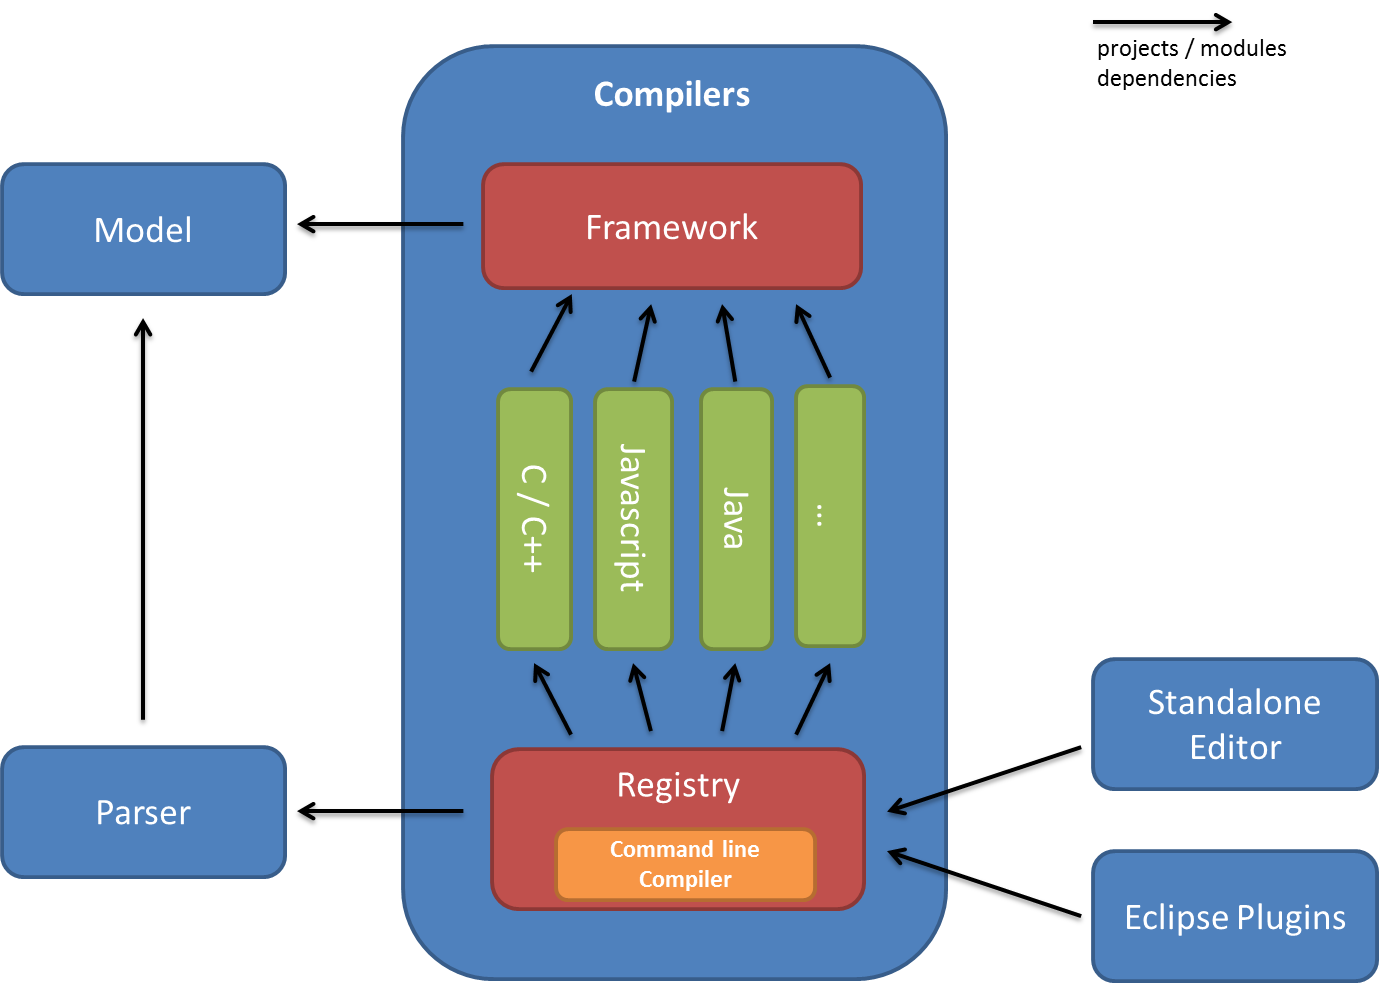
\includegraphics[width=\linewidth]{dsl.png}
	\caption{ThingML overview}
	\addloflink{https://heads-project.github.io/methodology/heads_methodology/extend_the_thingml_transformations_to_compile_code_for_a_new_platform.html}
  	\label{fig:thingml} 
\end{figure}

ThingML is used to describe state charts and components for an Internet of Things environment. The communication between models can be based on various asynchronous messaging protocols. ThingML is based on a modular and open-source platform. Therefore, there is an opportunity to contribute on the development and by the way adding extensions to the language.

\subsection{ThingML CEP Extension capabilities for Complex Event Processing}

As already mentioned, ThingML can be extended with various plug-in. The one which is focused in the article is the CEP extension. The article wrote by Lam An and Haugen Øystein defines the capability of ThingML to integrate a Complex Event Processing environment by answering to two questions.

\subsubsection{Is ThingML CEP Extension an efficient language for developing CEP applications ? }

The article answers to this question by evaluating the language expressiveness on two characteristics: the lines of codes and the number of keywords. The authors wrote different CEP operators using ThingML with and without CEP extension. The result is that there is less lines of codes and number of keywords by using the CEP extension but there isn't significant differences. However, this extension can be very useful in a large scale to save time by reducing those characteristics and in some cases a code duplication can be avoided. In a disjunction query for example, the non-usage of the CEP extension leads to check the occurrences of each event. This kind of situation conducts generally to code duplication and errors.

\subsubsection{Is ThingML CEP Extension powerful enough for CPS systems ? }

The article answers to this question by comparing ThingML CEP Extension with Esper which is an open source CEP Engine. The experiment done by the authors was base on the same workstation for all tests. They compared both technologies on Latency, CPU Utilization and Memory Utilization. The statistics show that ThingML with CEP extension uses less CPU and Memory than Esper. The CPU used by ThingML is around 50-60\% and 75-90\% for Esper. The Memory Usage is around 35-90MB for ThingML and 50-120MB for Esper. Nevertheless, the Esper latency is around 2 times faster than ThingML with CEP extension.

%----------------------------------------------------------------------------------------

\section{Conclusions}

In summary, ThingML CEP extension revealed to ease the creation of CEP applications than using ThingML without the CEP extension. The study also revealed that ThingML can be used with limited resources and shows reasonable latency for processing events. There is a need to evaluate ThingML with more complex systems to have more relevant informations. In fact, the authors tested those Frameworks with basic operations. They also tested it on a workstation with generous resources. It can be relevant to test ThingML on a Arduino or another physical limited workstation. 

\listoffigures

\printbibliography

\end{document}
